\iffalse
\let\negmedspace\undefined
\let\negthickspace\undefined
\documentclass[journal,12pt,twocolumn]{IEEEtran}
\usepackage{cite}
\usepackage{amsmath,amssymb,amsfonts,amsthm}
\usepackage{algorithmic}
\usepackage{graphicx}
\usepackage{textcomp}
\usepackage{xcolor}
\usepackage{txfonts}
\usepackage{listings}
\usepackage{enumitem}
\usepackage{mathtools}
\usepackage{gensymb}
\usepackage{comment}
\usepackage[breaklinks=true]{hyperref}
\usepackage{tkz-euclide} 
\usepackage{listings}
\usepackage{gvv}                                        
\def\inputGnumericTable{}                                 
\usepackage[latin1]{inputenc}                                
\usepackage{color}                                            
\usepackage{array}                                            
\usepackage{longtable}                                       
\usepackage{calc}                                             
\usepackage{multirow}                                         
\usepackage{hhline}                                           
\usepackage{ifthen}                                           
\usepackage{lscape}

\newtheorem{theorem}{Theorem}[section]
\newtheorem{problem}{Problem}
\newtheorem{proposition}{Proposition}[section]
\newtheorem{lemma}{Lemma}[section]
\newtheorem{corollary}[theorem]{Corollary}
\newtheorem{example}{Example}[section]
\newtheorem{definition}[problem]{Definition}
\newcommand{\BEQA}{\begin{eqnarray}}
\newcommand{\EEQA}{\end{eqnarray}}
\newcommand{\define}{\stackrel{\triangle}{=}}
\theoremstyle{remark}
\newtheorem{rem}{Remark}
\begin{document}

\bibliographystyle{IEEEtran}
\vspace{3cm}

\title{11.9.3.3}
\author{EE23BTECH11065 - prem sagar}
\maketitle
\newpage

\bigskip 

\renewcommand{\thefigure}{\theenumi}
\renewcommand{\thetable}{\theenumi}
\textbf{Question}:\\ The $5$th,$8$th and $11$th terms of a GP are p,q and s respectively .show that $q^2=ps$
\\\\\textbf{solution}:
\fi
\begin{table}[!ht]
   \centering
    \renewcommand\thetable{1}
      \begin{tabular}{|c|c|c|}
    \hline
            \textbf{Symbol} & \textbf{Value} & \textbf{Description} \\
    \hline
          $x\brak{5}$ & $p$ & $x\brak{0}r^5$ \\
    \hline
          $x\brak{8}$ & $q$ & $x\brak{0}r^8$\\
    \hline 
          $x\brak{{11}}$ &$s$ &$x\brak{0}r^{11}$ \\
    \hline
          $x\brak{n}$ & &$x\brak{0}r^nu\brak{n}$ \\
    \hline
          $r$& $\brak{\frac{s}{p}}^\frac{1}{6}$& common ratio\\
     \hline     
  \end{tabular}

    \caption{input parameters}
    \label{tab:11.9.3}
 \end{table}
 From \tabref{tab:11.9.3}:
\begin{align}
q^2&=x\brak{0}\,r^8\,x\brak{0}\,r^8
     \\ &=x\brak{0}^2\,r^{16}
\\ps&=x\brak{0}\,r^5\,x(0)\,r^{11}
       \\&=x\brak{0}^2\,r^{16}
\\\implies q^2&=ps
\end{align}
now we will find r and x\brak{0}:
\begin{align}
\frac{s}{p}&=\frac{x\brak{0}r^{11}}{x\brak{0}r^5}
\\r&=\brak{\frac{s}{p}}^\frac{1}{6} 
\\p&=x\brak{0}\brak{\frac{s}{p}}^\frac{5}{6}
\\x\brak{0}&=\frac{p^\frac{11}{6}}{s^\frac{5}{6}}
\end{align}
Applying z-Transform:
\begin{align}
     X(z) &= \frac{x\brak{0}}{1-r\,z^{-1}}\: \:,\abs{z}>\abs{r}
\\ \implies  X(z)&=\frac{p^3}{p^\frac{7}{6}s^\frac{5}{6}-q^2z^{-1}}\:,\abs{z}>\abs{\brak{\frac{q}{p}}^\frac{1}{3}}
     \end{align}    
\\\begin{figure}[h]
   \renewcommand\thefigure{1}
    \centering
    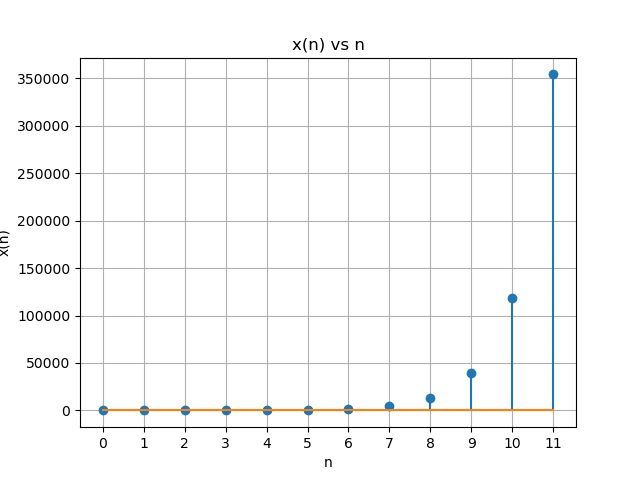
\includegraphics[width=1\linewidth]{ncert-maths/11/9/3/3/figs/figure__plot.png}
    \caption{plot x\brak{n}vs n\hspace{0.1cm}$p=486$,
    \hspace{0.1cm}$q=13122$,
    \hspace{0.1cm}$s=354294$,
    \hspace{0.1cm}$r=3$}
    \label{fig:1}
\end{figure}
